\subsection{Closed fuel cycles}
\begin{frame}
    \frametitle{What about a different fuel cycle option?}
    What if we had a closed fuel cycle that required \gls{HALEU}?
    \begin{itemize}
        \item How does the fuel cycle option impact the material requirements?
        \item Does this save resources?
    \end{itemize}

\end{frame}

\begin{frame}
    \frametitle{Reactor models account for fuel depletion}
    \begin{itemize}
    \item \Cyclus uses archetypes to model reactors, and the physics 
        of a reactor
    \item Different reactor archetypes use different methodologies 
        to model fuel depletion
   \item<2-> The \Cycamore \texttt{Reactor} uses recipes to define spent fuel compositions
   \item<2-> Other \Cyclus reactor archetypes can dynamically model 
         fuel depletion, but they require export controlled software 
         or are reactor design specific
    \item<3-> \Gls{SNF} compositions impact numerous fuel cycle considerations:
    \begin{itemize}
        \item<3-> decay heat
        \item<3-> criticality safety
        \item<3-> amount of plutonium and transuranic elements
    \end{itemize}


\end{itemize}
\end{frame}

\begin{frame}
    \frametitle{OpenMCyclus: an open source coupling with OpenMC}
    \begin{columns}
        \column[t]{5cm}
    \begin{itemize}
        \item Developed a reactor archetype that couples \Cyclus with 
              stand-alone depletion solver in OpenMC
        \item Publicly available on GitHub \cite{bachmann_openmcyclus_2023}
        \item<2-> Compared against the \Cycamore \texttt{Reactor} in a 
              simple closed fuel cycle
    \end{itemize}

    \column[t]{6.5cm}\begin{figure}[h!]
        \centering
        \small
        \begin{tikzpicture}[node distance=2cm]
            \node (dre) [facility] {Dynamic resource exchange};
            \node (fresh) [facility, below of=dre, xshift=-2.5cm,text width=1cm]{Fresh fuel inventory};
            \node (core) [facility, below of=dre, text width=1cm]{Core inventory};
            \node (spent) [facility, below of=dre, xshift=2.5cm,text width=1cm]{Spent fuel inventory};
            \node (openmc) [facility, below of=core]{OpenMC};

            \draw [arrow] (dre) -- node[anchor=east, text width=1cm]{Fresh fuel} (fresh);
            \draw [arrow] (dre) -- node[anchor=east, text width=1cm,pos=0.7]{Fresh fuel} (core);
            \draw [arrow] (fresh) -- node[anchor=north, text width=1cm]{Fresh fuel} (core);
            \draw [arrow] (core) -- node[anchor=north, text width=1cm]{Depleted fuel} (spent);
            \draw [arrow] (spent) -- node[anchor=west, text width=1cm]{Spent fuel} (dre);
            \draw [<->] (core) -- node[anchor=west, text width=1cm]{Compositions} (openmc);
            \end{tikzpicture}
        \caption{Material handling pathways between different material 
        inventories in OpenMCyclus and the \gls{DRE} of \Cyclus. }
        \label{fig:openmcyclus-flow}
    \end{figure}

    \end{columns}
\end{frame}

\begin{frame}
    \frametitle{Benchmark description}
    \begin{columns}
        \column[t]{4.5cm}
        \begin{itemize}
            \item Closed fuel cycle with 1 reactor type, modeled with 
                  either \Cycamore or OpenMCyclus
            \item Reactors prefer MOX over UOX
            \item<2-> 2 reactors deployed at time step 1, then 1 deployed at 
                  time steps 50, 100, 150
            \item<2-> Reactors have 60 time step lifetime
            \item<3-> Ran with \Cycamore \texttt{Reactor} twice, toggling 
                  the \texttt{decom\_transmute\_all} setting
        \end{itemize}
        \column[t]{6.3cm}
        \begin{figure}
            \centering
            \small
            \begin{tikzpicture}[node distance=1cm]
                \node (mine) [facility] {Uranium Mine};
                \node (enrichment) [facility, below of=mine]{Enrichment};
                \node (reactor) [facility, below of=enrichment]{Reactor};
                \node (sinkhlw) [facility, below of=reactor, xshift=1.5cm, yshift=-0.5cm]{Repository};
                \node (separation) [facility, right of=reactor, xshift=2.2cm]{Separations};
                \node (mox_fab) [facility, above of=separation, yshift=0.4cm]{MOX Fuel Fab};
                
                \draw [arrow] (mine) -- node[anchor=east]{Natural U} (enrichment);
                \draw [arrow] (enrichment) -- node[anchor=east]{Fresh UOX}(reactor);
                \draw [arrow] (reactor) -- node[anchor=north]{Spent UOX}(separation);
                \draw [arrow] (separation) -- node[anchor=west, text width=0.5cm]{Separated Pu}(mox_fab);
                \draw [arrow] (separation) |- node[anchor=west, text width=0.5cm, pos=0.3]{Fission products}(sinkhlw);
                \draw [arrow] (mine) -| node[anchor=south, pos=0.4]{Natural U} (mox_fab);
                \draw [arrow] (reactor) |- node[anchor=east, pos=0.3]{Spent MOX} (sinkhlw);
                \draw [arrow] (mox_fab) -- node[anchor=south, sloped]{Fresh MOX} (reactor);
                \end{tikzpicture}
            \caption{Fuel cycle facilities and material flow between facilities for the 
            sample fuel cycle scenarios used to compare the results of the \Cycamore Reactor 
            and OpenMCyclus DepleteReactor archetypes. }
            \label{fig:comparison}
        \end{figure}
    \end{columns}
\end{frame}

\begin{frame}
    \frametitle{Benchmark Results (I)}
    \begin{columns}
        \column[t]{3.8cm}
        \begin{itemize}
            \item Separated plutonium masses differ because of 
                  different depletion methodologies
            \begin{itemize}
                \item<2-> \Cycamore \texttt{Reactor} applies the same 
                          SNF composition
                \item<2-> OpenMCyclus depletes fuel on a per cycle basis
            \end{itemize}
        \end{itemize}
        \column[t]{6.5cm}
        \begin{figure}
            \centering 
            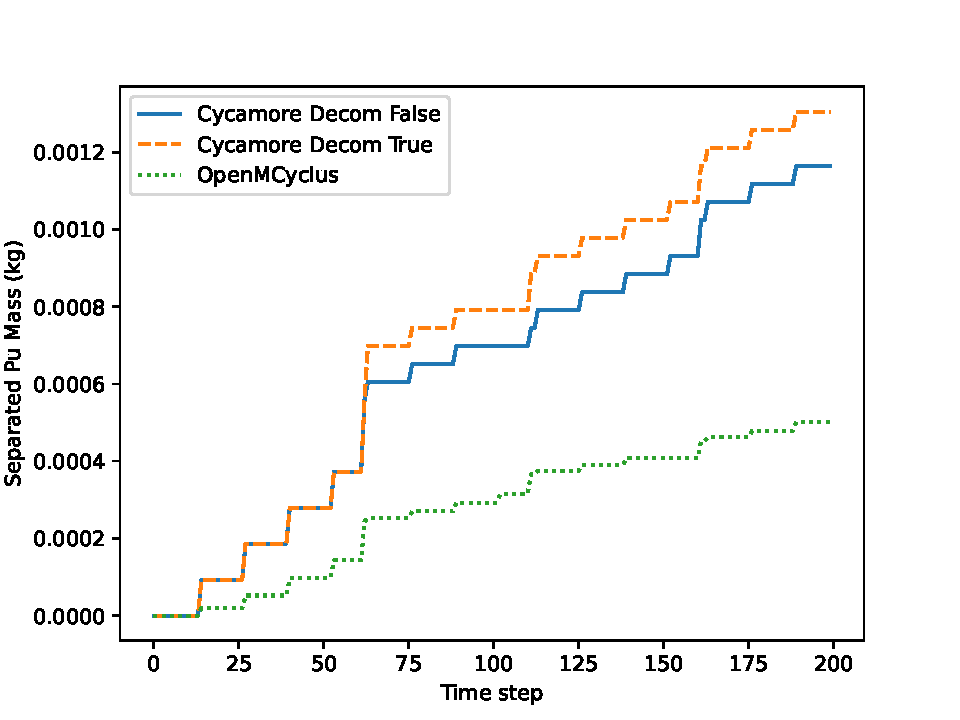
\includegraphics[scale=0.42, trim=0 0 0 30,clip]{comparison_pu_cumulative.pdf}
            \caption{Comparison of cumulative separated plutonium in benchmark between 
            OpenMCyclus and \Cycamore \texttt{Reactor}.}
        \end{figure}
    \end{columns}
\end{frame}

\begin{frame}
    \frametitle{Benchmark Results (I)}
    \begin{columns}
        \column[t]{3.8cm}
        \begin{itemize}
            \item Separated plutonium masses differ because of 
                  different depletion methodologies
                  \begin{itemize}
                    \item \Cycamore \texttt{Reactor} applies the same 
                          SNF composition
                    \item OpenMCyclus depletes fuel on a per cycle basis
                  \end{itemize}
            \item Temporarily changing OpenMCyclus method shows better agreement
            \item<2-> Results suggests \Cycamore \texttt{Reactor} overestimates 
                  separated plutonium inventory
        \end{itemize}
        \column[t]{6.5cm}
        \begin{figure}
            \centering 
            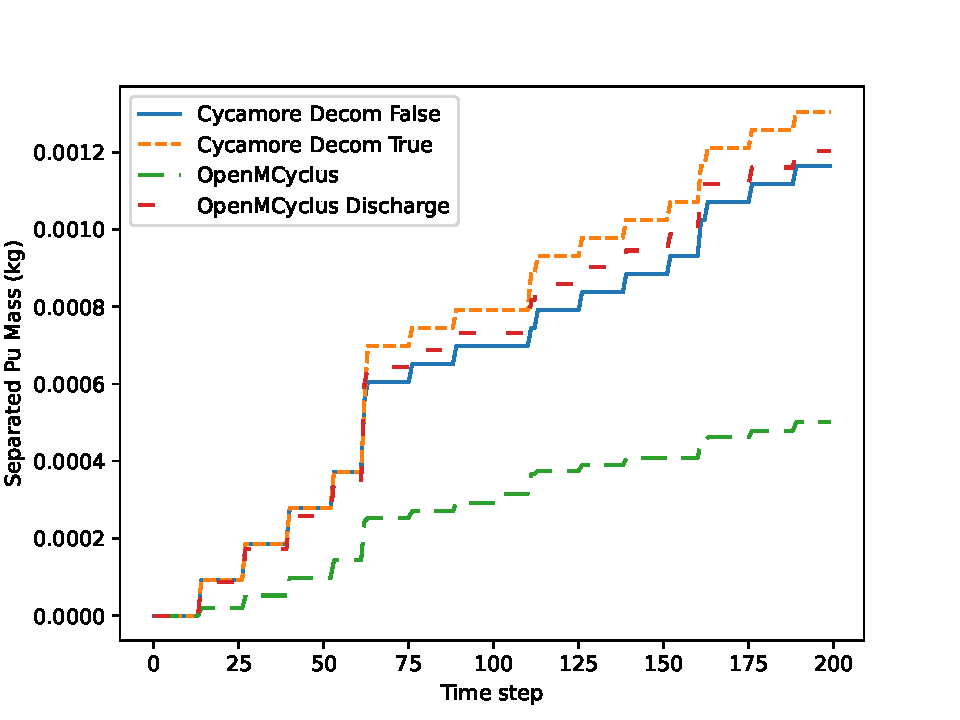
\includegraphics[scale=0.42, trim=0 0 0 30,clip]{comparison_pu_cumulative_discharge.pdf}
            \caption{Comparison of cumulative separated plutonium in benchmark between 
            OpenMCyclus and \Cycamore \texttt{Reactor}.}
        \end{figure}
    \end{columns}
\end{frame}

\begin{frame}
    \frametitle{Benchmark Results (II)}
        \begin{itemize}
            \item Differences in separated plutonium masses 
                  propagate into different fuel receipts 
            \item Spent fuel masses are mostly consistent, except 
                  when a reactor is decommissioned
        \end{itemize}
        \begin{figure}
            \centering
            \begin{subfigure}{0.48\textwidth}
                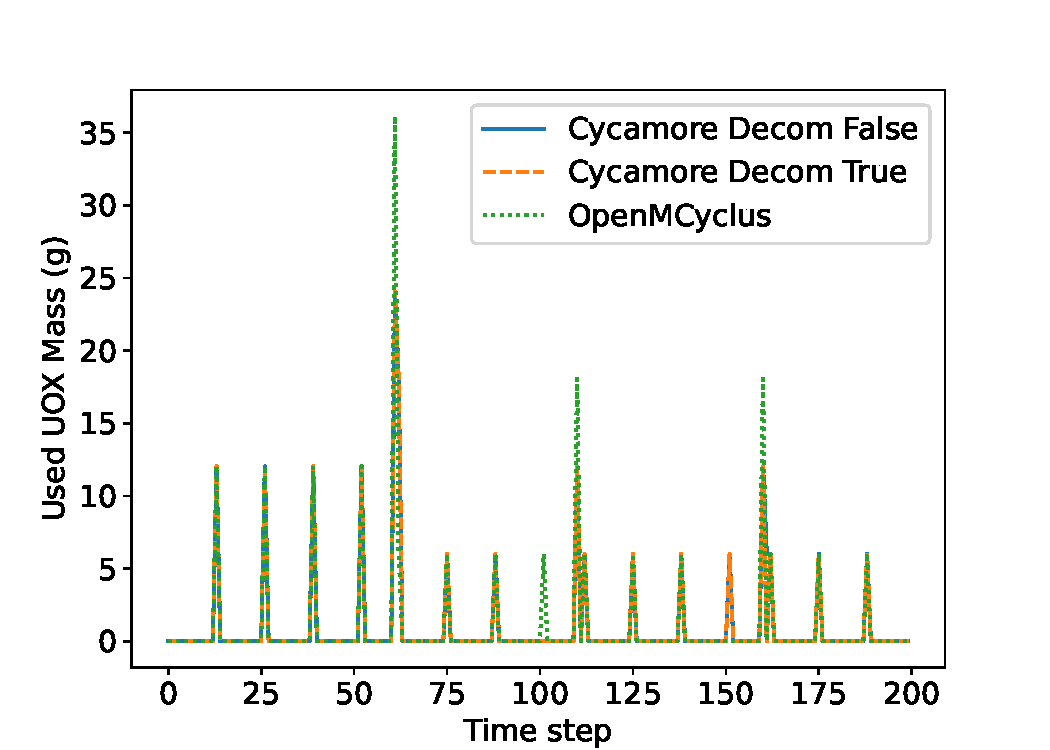
\includegraphics[width=\linewidth]{comparison_spentuox.pdf}
                \caption{Comparison of Spent UOX fuel discharged.}
            \end{subfigure}
            \hfill
            \begin{subfigure}{0.48\textwidth}
                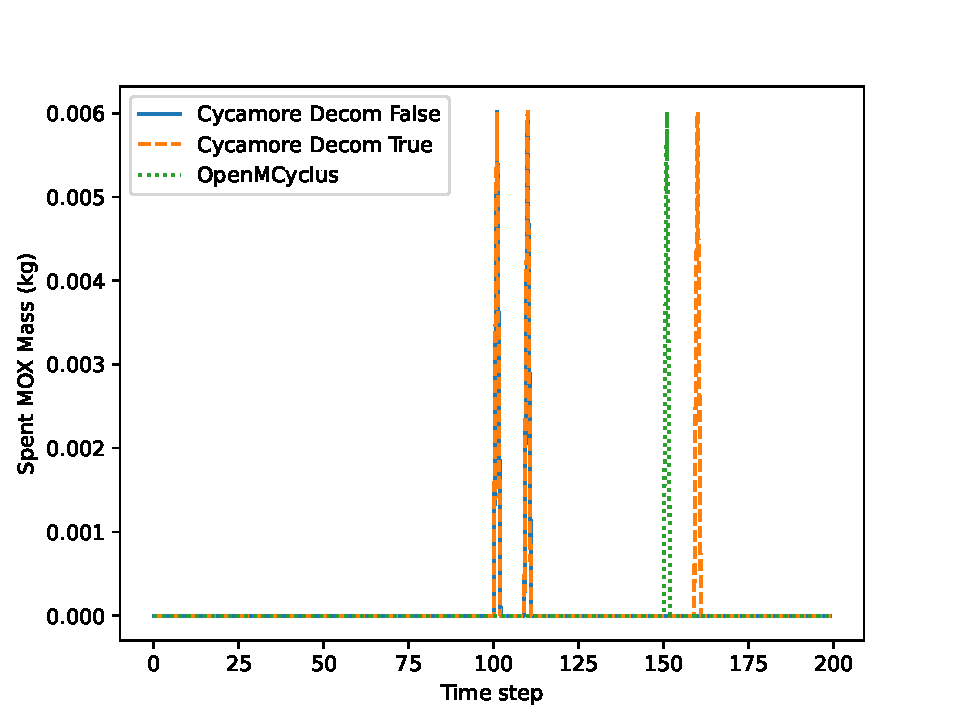
\includegraphics[width=\linewidth]{comparison_spentmox.pdf}
                \caption{Comparison of Spent MOX fuel discharged.}
            \end{subfigure}
            \caption{Spent fuel transactions in OpenMCyclus/\Cycamore benchmark}
            \label{fig:spentfuel_benchmark}
        \end{figure}

\end{frame}

\begin{frame}
    \frametitle{Recycle scenario definitions}
    \begin{table}[ht]
        \centering
        \caption{Summary of the recycle fuel cycle transition scenarios.
        Energy growth is relative to energy from \glspl{LWR} in 2025}
        \label{tab:scenarios_recycle}
        \begin{tabular}{c l l l}
            \hline
            Scenario & Advanced Reactors & Energy demand & Recycle scheme\\\hline
            \rowcolor{lightgray}14 & Xe-100, MMR, VOYGR & No growth & Limited \\
            \rowcolor{lightgray}15 & Xe-100, MMR, VOYGR & No growth & Limited, no TRISO\\
            \rowcolor{lightgray}16 & Fast reactor & No growth & Continuous \\
            \rowcolor{lightpink}17 & Xe-100, MMR, VOYGR & 1\% growth & Limited \\
            \rowcolor{lightpink}18 & Xe-100, MMR, VOYGR & 1\% growth & Limited, no TRISO\\
            \rowcolor{lightpink}19 & Fast reactor & 1\% growth & Continuous\\
            \hline
    \end{tabular}
    \end{table}
        %<2-> \tikz[overlay, remember picture]{\draw{draw=red,thick, double, fillopacity=0.2] ($(infrastructure)+(-0.5,0.4)$) rectangle ($(infrastructure)+(6,-0.2)$);}} 
\end{frame}

\begin{frame}
    \frametitle{Recycle scenario definitions}
        \begin{table}[ht]
            \centering
            \caption{Summary of the recycle fuel cycle transition scenarios.
            Energy growth is relative to energy from \glspl{LWR} in 2025}
            \label{tab:scenarios_recycle_box}
            \begin{tabular}{c l l l}
                \hline
                Scenario & Advanced Reactors & Energy demand & Recycle scheme\\\hline
                \rowcolor{lightgray}\marktopleft{a3}14 & Xe-100, MMR, VOYGR & No growth & Limited \\
                \rowcolor{lightgray}15 & Xe-100, MMR, VOYGR & No growth & Limited, no TRISO\\
                \rowcolor{lightgray}16 & Fast reactor& No growth & Continuous~~~~~~~~\markbottomright{a3}\\
                \rowcolor{lightpink}17 & Xe-100, MMR, VOYGR& 1\% growth & Limited \\
                \rowcolor{lightpink}18 & Xe-100, MMR, VOYGR & 1\% growth & Limited, no TRISO\\
                \rowcolor{lightpink}19 & Fast reactor & 1\% growth & Continuous\\
                \hline
        \end{tabular}
        \end{table}
\end{frame}




\begin{frame}
    \frametitle{Limited recycle fuel cycle assumptions}
    \begin{columns}
        
    \column[t]{6cm}
    \vspace{-0.6cm}
    \begin{figure}
    \centering
    \begin{tikzpicture}[node distance=0.85cm]
        \node (mine) [facility] {\tiny Uranium Mine};
        \node (enrichment) [facility, below of=mine]{\tiny Enrichment};
        \node (reactor) [facility, below of=enrichment]{\tiny Reactor};
        \node (adv_reactor) [transition, right of=reactor, xshift=1.3cm]{\tiny Advanced Reactor};
        \node (wetstorage) [facility, below of=reactor]{\tiny Wet Storage};
        \node (drystorage) [facility, below of=wetstorage]{\tiny Dry Storage};
        \node (cooling) [transition, below of=adv_reactor]{\tiny Cooling Pool};
        \node (sinkhlw) [facility, below of=drystorage, xshift=1cm]{\tiny HLW Sink};
        \node (sinkllw) [facility, left of=enrichment, xshift=-1cm]{\tiny LLW Sink};
        \node (separation) [transition, below of=cooling]{\tiny Separations};
        \node (fuelfab) [transition, below of=adv_reactor,xshift=1.3cm]{\tiny Fuel Fab};
        
        \draw [arrow] (mine) --(enrichment);
        \draw [arrow] (enrichment) -- (reactor);
        \draw [arrow] (enrichment) -- (sinkllw);
        \draw [arrow] (enrichment) -| (adv_reactor);
        \draw [arrow] (reactor) -- (wetstorage);
        \draw [arrow] (wetstorage) -- (drystorage);
        \draw [arrow] (drystorage) |- (sinkhlw);
        \draw [arrow] (adv_reactor) -- (cooling);
        \draw [dashed, ->] (cooling) -- (separation);
        \draw [arrow] (separation) -| (fuelfab);
        \draw [arrow] (fuelfab) |- (adv_reactor);
        \draw [arrow] (separation) |- (sinkhlw);
        \draw [arrow] (wetstorage) -- (separation);
        \draw [dashed, ->] (cooling) -| (sinkhlw);

        \end{tikzpicture}
    \caption{Fuel cycle facilities and material flow between facilities for the recycling 
    scenarios.}
    \label{fig:limited_fuel_cycle}
\end{figure}

        \column[t]{4.5cm}
        \vspace{-0.5cm}
        \begin{itemize}
            \item Reprocess uranium-based fuel, dispose plutonium-based fuel
            \item Reactors prefer plutonium-based fuel over uranium-based fuel
            \item Separations remove only plutonium (aqueous reprocessing)
            \item<2-> Use the same deployment schedule as Scenarios 7, 13
            \item<2-> Modeled Xe-100 and VOYGR with OpenMCyclus
            \item<3-> Separations start in 2020
            \item<3-> Vary if \gls{TRISO} \gls{SNF} is reprocessed
        \end{itemize}

\end{columns}
\end{frame}

\begin{frame}
    \frametitle{Continuous recycle fuel cycle assumptions}
    \begin{columns}
        
    \column[t]{6cm}
    \vspace{-0.5cm}
    \begin{figure}
    \centering
    \begin{tikzpicture}[node distance=1.2cm]
        \node (mine) [facility] {Uranium Mine};
        \node (enrichment) [facility, below of=mine]{Enrichment};
        \node (reactor) [facility, below of=enrichment]{Reactor};
        \node (wetstorage) [facility, below of=reactor, text width=1.2cm]{Cooling Pool};
        \node (sinkhlw) [facility, below of=wetstorage, xshift=1.2cm]{Repository};
        \node (separation) [transition, right of=wetstorage,xshift=1cm]{Separations};
        \node (fuelfab) [transition, above of=separation]{Fuel Fab};
        %\node (fr_enrichment) [transition, right of=enrichment,xshift=3cm, text width=1.2cm]{FR Enrichment};
        \node (sfr) [transition, right of=fuelfab, xshift=1.cm,text width=1.2cm]{Fast Reactor};
        
        \draw [arrow] (mine) -- (enrichment);
        \draw [arrow] (enrichment) -- (reactor);
        \draw [arrow] (reactor) -- (wetstorage);
        \draw [arrow] (wetstorage) |- (sinkhlw);
        \draw [arrow] (separation) -- (fuelfab);
        \draw [arrow] (separation) -- (sinkhlw);
        \draw [arrow] (fuelfab) -- (sfr);
        \draw [dashed, ->] (wetstorage) -- (separation);
        \draw [arrow] (sfr) |- (separation);
        \draw [arrow] (enrichment) -| (sfr);

        \end{tikzpicture}
    \caption{Fuel cycle facilities and material flow between facilities for 
    the continuous recycling scenarios.}
    \label{fig:continuous_fuel_cycle}
\end{figure}

        \column[t]{4.5cm}
        \begin{itemize}
            \item Reprocess all \gls{SNF} 
            \item Introduce a fast reactor for transition, modeled through 
                  OpenMCyclus
            \item Separation start 2020
            \item Can accept plutonium-based fuel (preferred) or \gls{HALEU}
            \item Separations remove U, Np, Pu, Am (electrochemical reprocessing)
            \item<2-> Use the same deployment scheme to determine how many fast 
                  reactors to deploy
        \end{itemize}

\end{columns}
\end{frame}

\begin{frame}
    \frametitle{Advanced reactors}
    \vspace{-0.7cm}
    \begingroup
        \renewcommand{\arraystretch}{1.2}
        \begin{table}
            \centering
            \begin{threeparttable}
        
            \caption{Fast reactor design specification.}
            \label{tab:fast_rx}
            \begin{tabular}{l c}
                \hline
                Design Criteria & Fast Reactor \cite{fichtlscherer_assessing_2019,triplett_prism:_2012}\\
                \hline
                Reactor type & \acrfull{SFR} \\
                Fuel form &  Metallic \\
                Power Output (MWe) & 311 \\
                Power Output (MWth) & 840 \\
                Enrichment (wt\% fissile Pu) &  11.3/13.5\\
                Cycle Length (yrs) & 1 \\
                Number of cycles &  4 \\
                Reactor Lifetime (yrs)&  60\\
                Burnup (MWd/kg) & 87.51 \\
                \hline
            \end{tabular}
        \end{threeparttable}
        \end{table} 
    \endgroup
\end{frame}
